\chapter{Background Appendix}
% \begin{figure}[ht!]
%     \centering
%     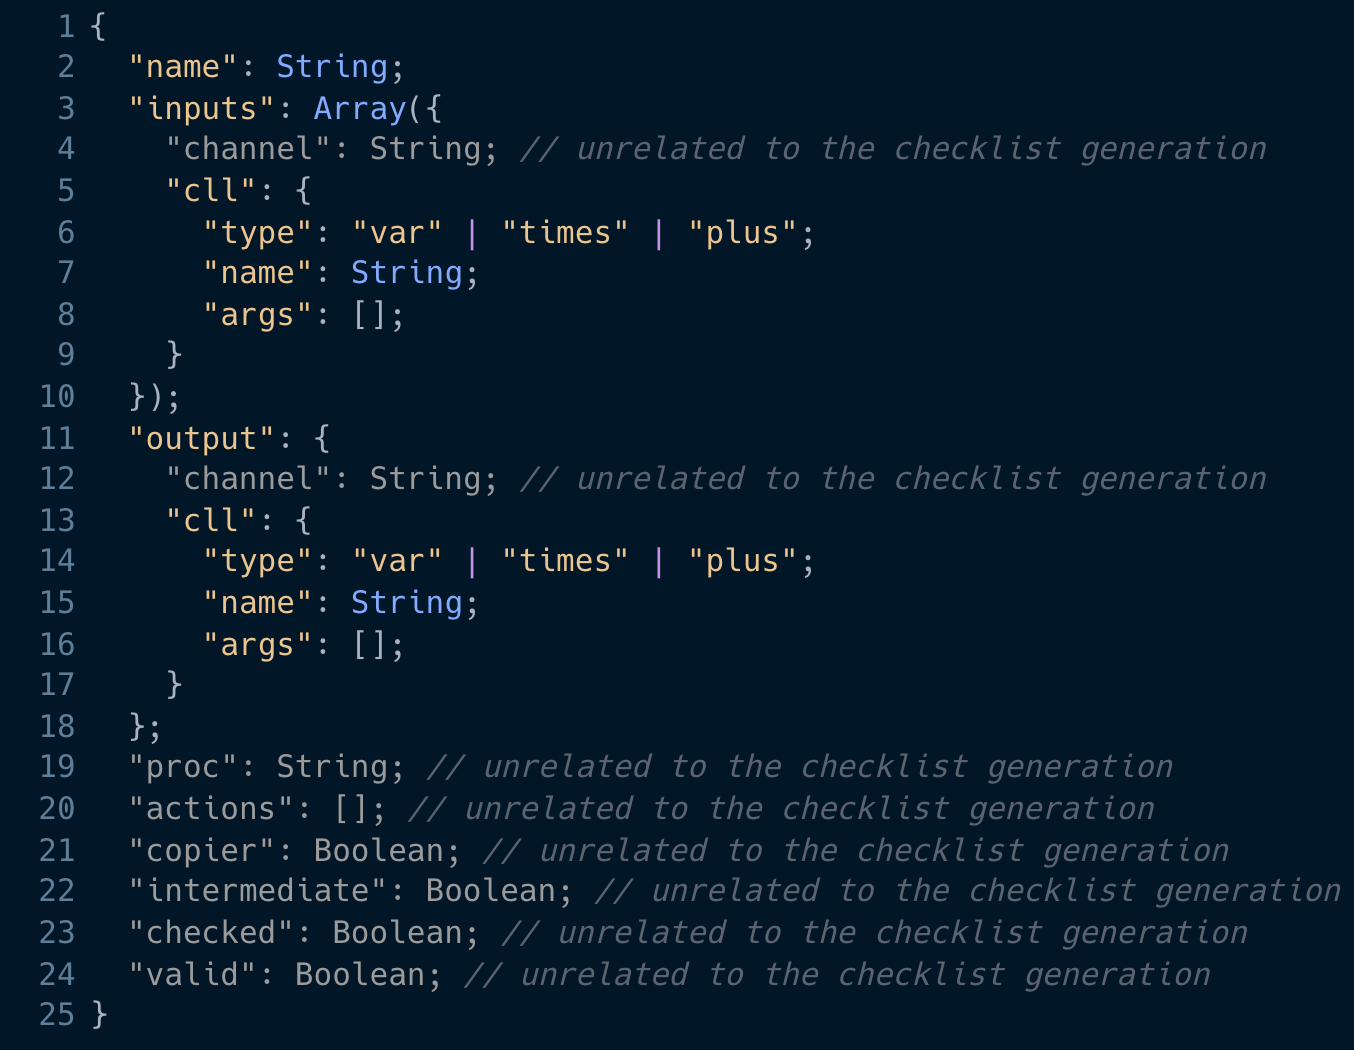
\includegraphics[width=0.85\textwidth]{overleaf/images/workflowfm_json.png}
%     \caption{WorkflowFM's Process JSON}
%     \label{appendix:fig:workflowfm_json}
% \end{figure}

\begin{figure}
    \centering
    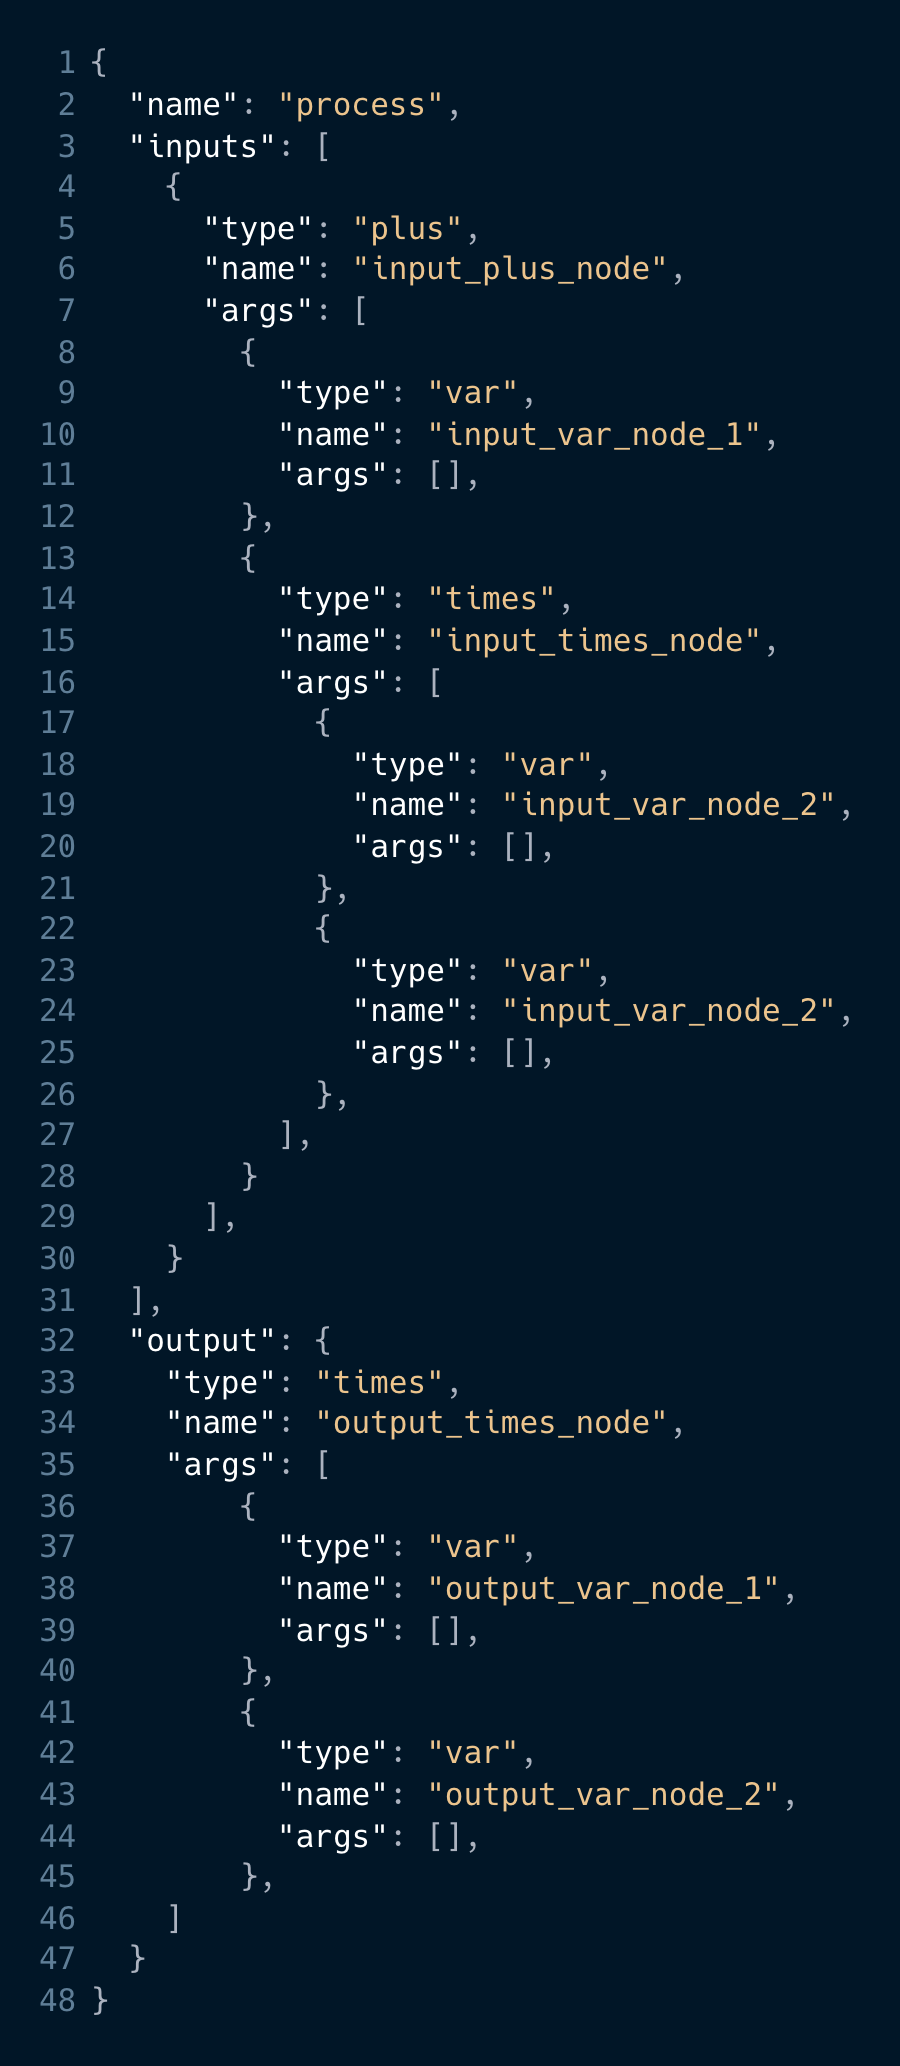
\includegraphics[width=0.65\textwidth]{overleaf/images/example_json.png}
    \caption{Figure \ref{fig:process_flows}'s JSON}
    \label{appendix:fig:example_json}
\end{figure}

\chapter{Design Appendix}
\begin{figure}[ht!]
    \centering
    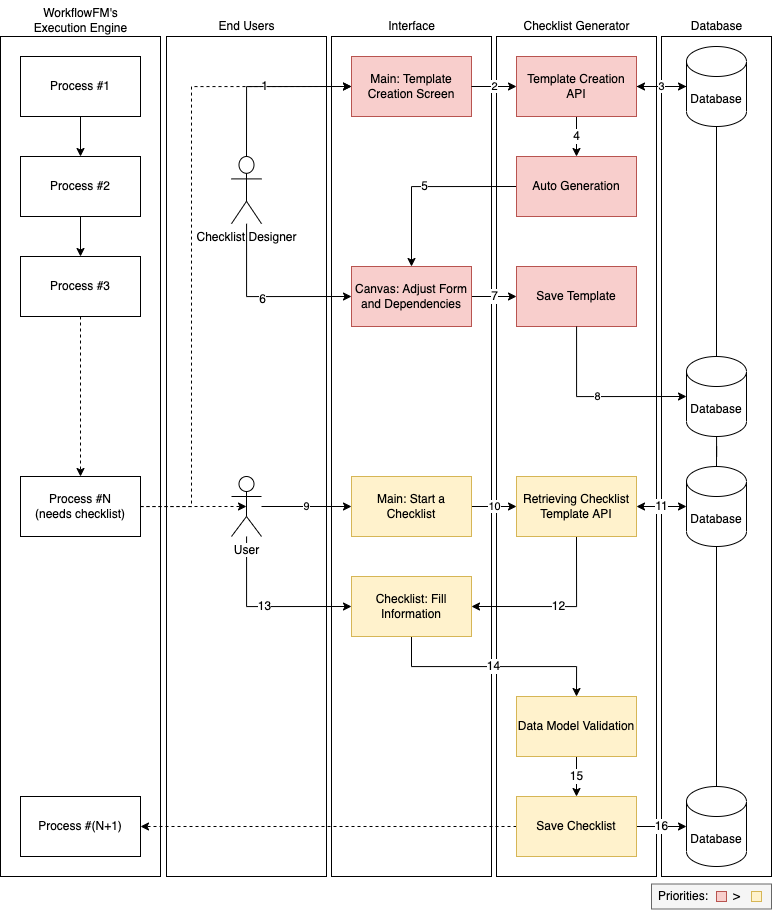
\includegraphics[width=\textwidth]{overleaf/images/overall_system_diagram_full.png}
    \caption{Detailed Overall System Diagram}
    \label{appendix:fig:overall_system_diagram}
\end{figure}


\begin{figure}[ht]
    \centering
    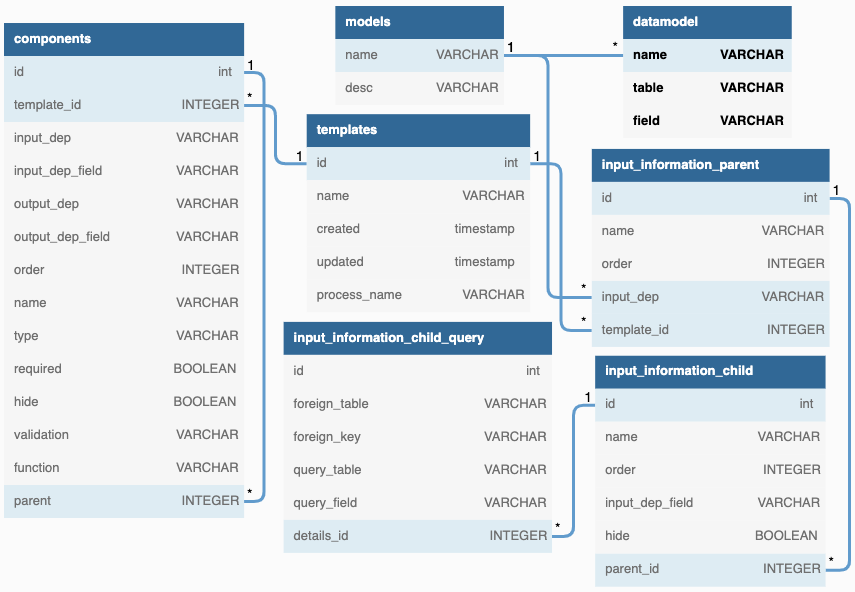
\includegraphics[width=\textwidth]{overleaf/images/checklist_db_design.png}
    \caption{Checklist Database Design}
    \label{fig:checklist_db_design}
\end{figure}

\chapter{Sequence Diagrams}
\label{appendix:sequence_diagrams}
\begin{figure}[ht!]
    \centering
    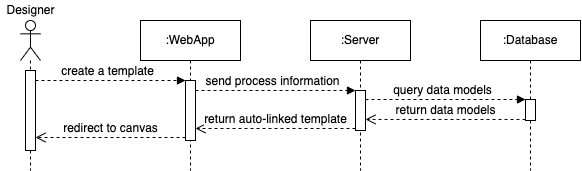
\includegraphics[width=\textwidth]{overleaf/images/create_template.png}
    \caption{Sequence Diagram of Create Template Scenario}
    \label{fig:create_template}
\end{figure}

\noindent
\textbf{Scenario \#1:} Figure \ref{fig:create_template} \\
\textbf{Goal:} \\
\textbf{Preconditions:} \\
\textbf{Breakdown:} \\

\begin{figure}[ht!]
    \centering
    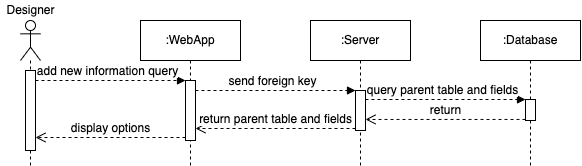
\includegraphics[width=\textwidth]{overleaf/images/add_new_information_query.png}
    \caption{Sequence Diagram of Add New Information Query Scenario}
    \label{fig:add_new_information_query}
\end{figure}

\noindent
\textbf{Scenario \#2:} Figure \ref{fig:add_new_information_query} \\
\textbf{Goal:} \\
\textbf{Preconditions:} \\
\textbf{Breakdown:} \\

\begin{figure}[ht!]
    \centering
    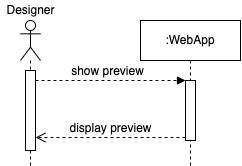
\includegraphics[width=0.4\textwidth]{overleaf/images/show_preview.png}
    \caption{Sequence Diagram of Show Preview Scenario}
    \label{fig:show_preview}
\end{figure}

\noindent
\textbf{Scenario \#3:} Figure \ref{fig:show_preview} \\
\textbf{Goal:} \\
\textbf{Preconditions:} \\
\textbf{Breakdown:} \\

\begin{figure}[ht!]
    \centering
    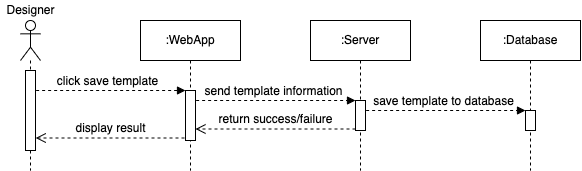
\includegraphics[width=\textwidth]{overleaf/images/save_template.png}
    \caption{Sequence Diagram of Save Template Scenario}
    \label{fig:save_template}
\end{figure}

\noindent
\textbf{Scenario \#4:} Figure \ref{fig:save_template} \\
\textbf{Goal:} \\
\textbf{Preconditions:} \\
\textbf{Breakdown:} \\

\begin{figure}[ht!]
    \centering
    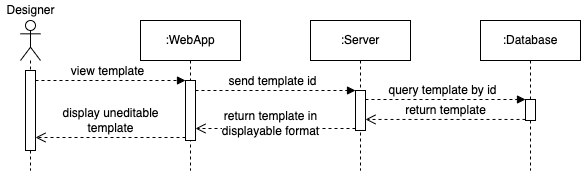
\includegraphics[width=\textwidth]{overleaf/images/view_template.png}
    \caption{Sequence Diagram of View Template Scenario}
    \label{fig:view_template}
\end{figure}

\noindent
\textbf{Scenario \#5:} Figure \ref{fig:view_template} \\
\textbf{Goal:} \\
\textbf{Preconditions:} \\
\textbf{Breakdown:} \\



\chapter{Participants' information sheet}
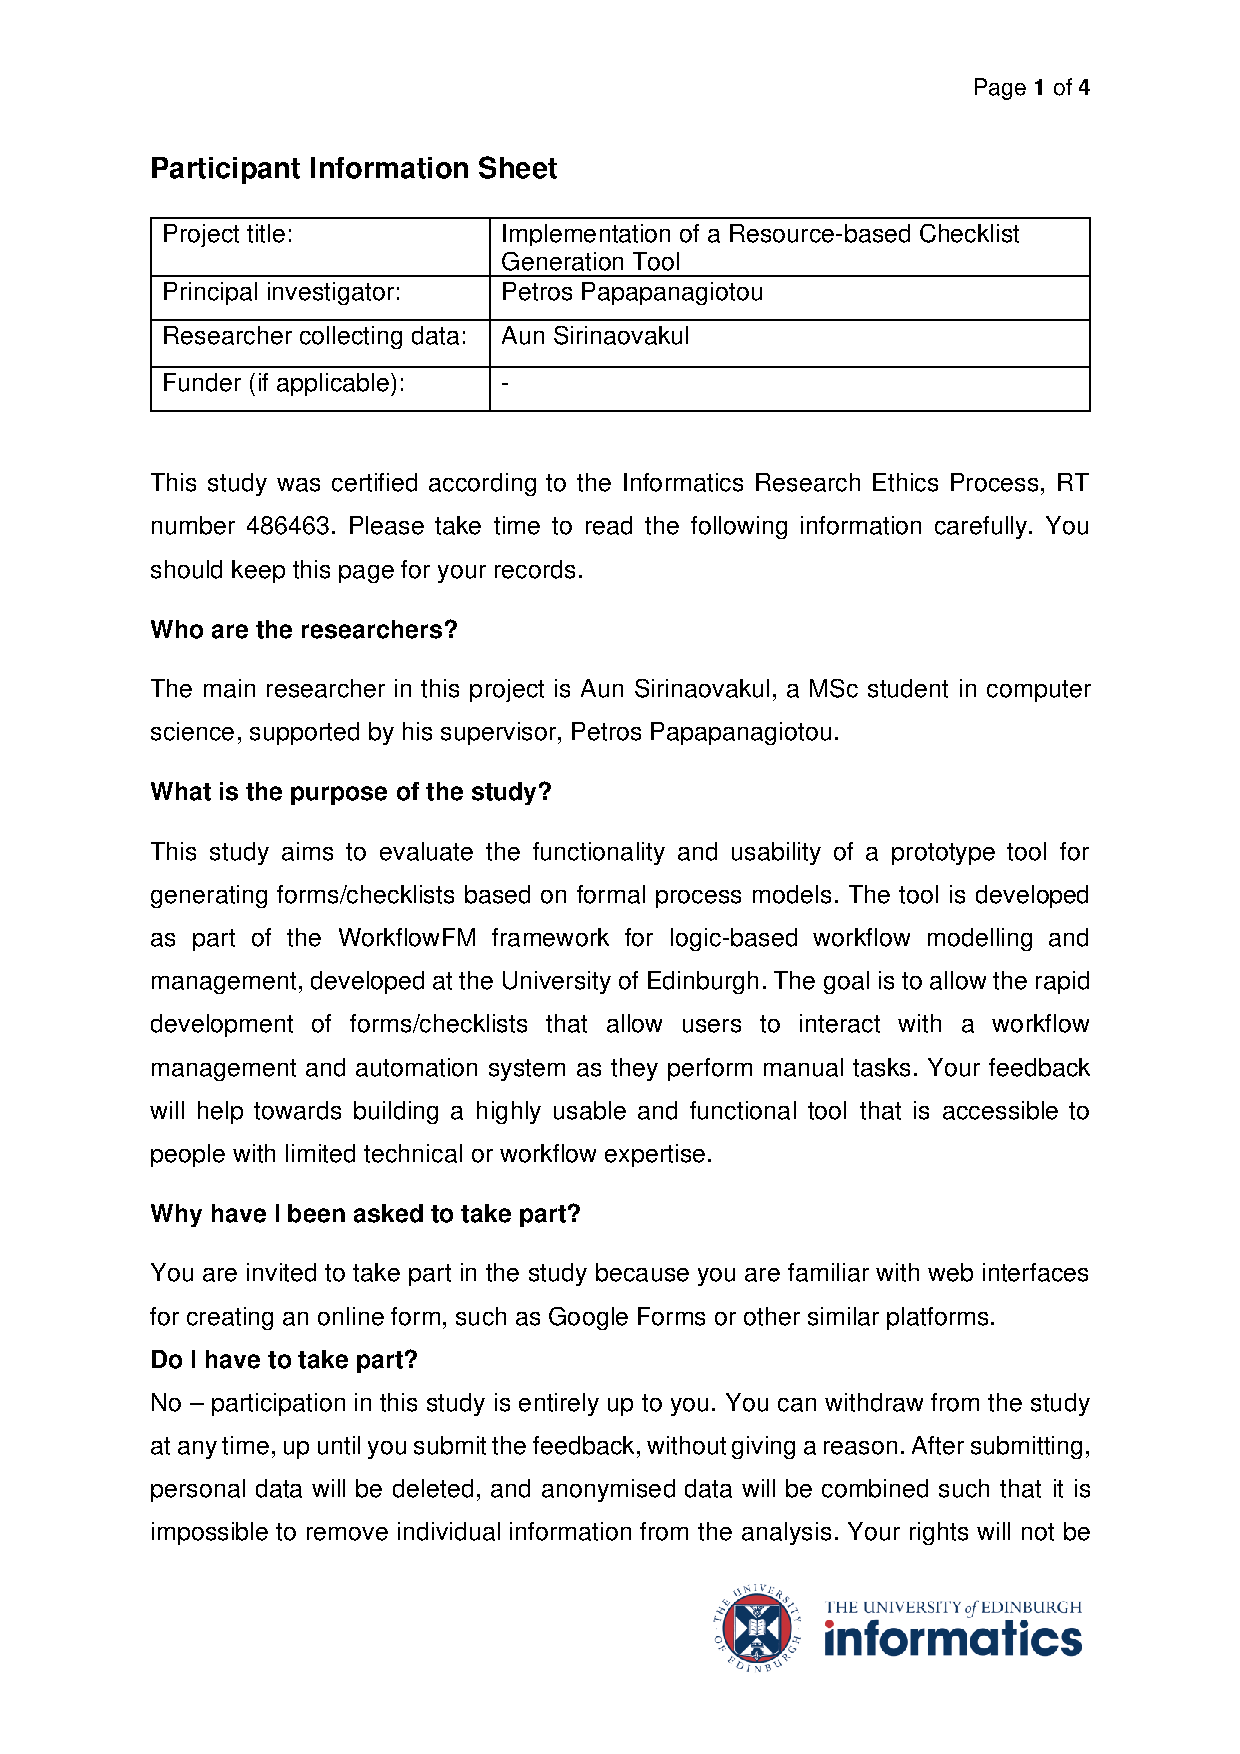
\includepdf[pages=-]{./pdf/Participant Information Sheet .pdf}

\chapter{Participants' consent form}
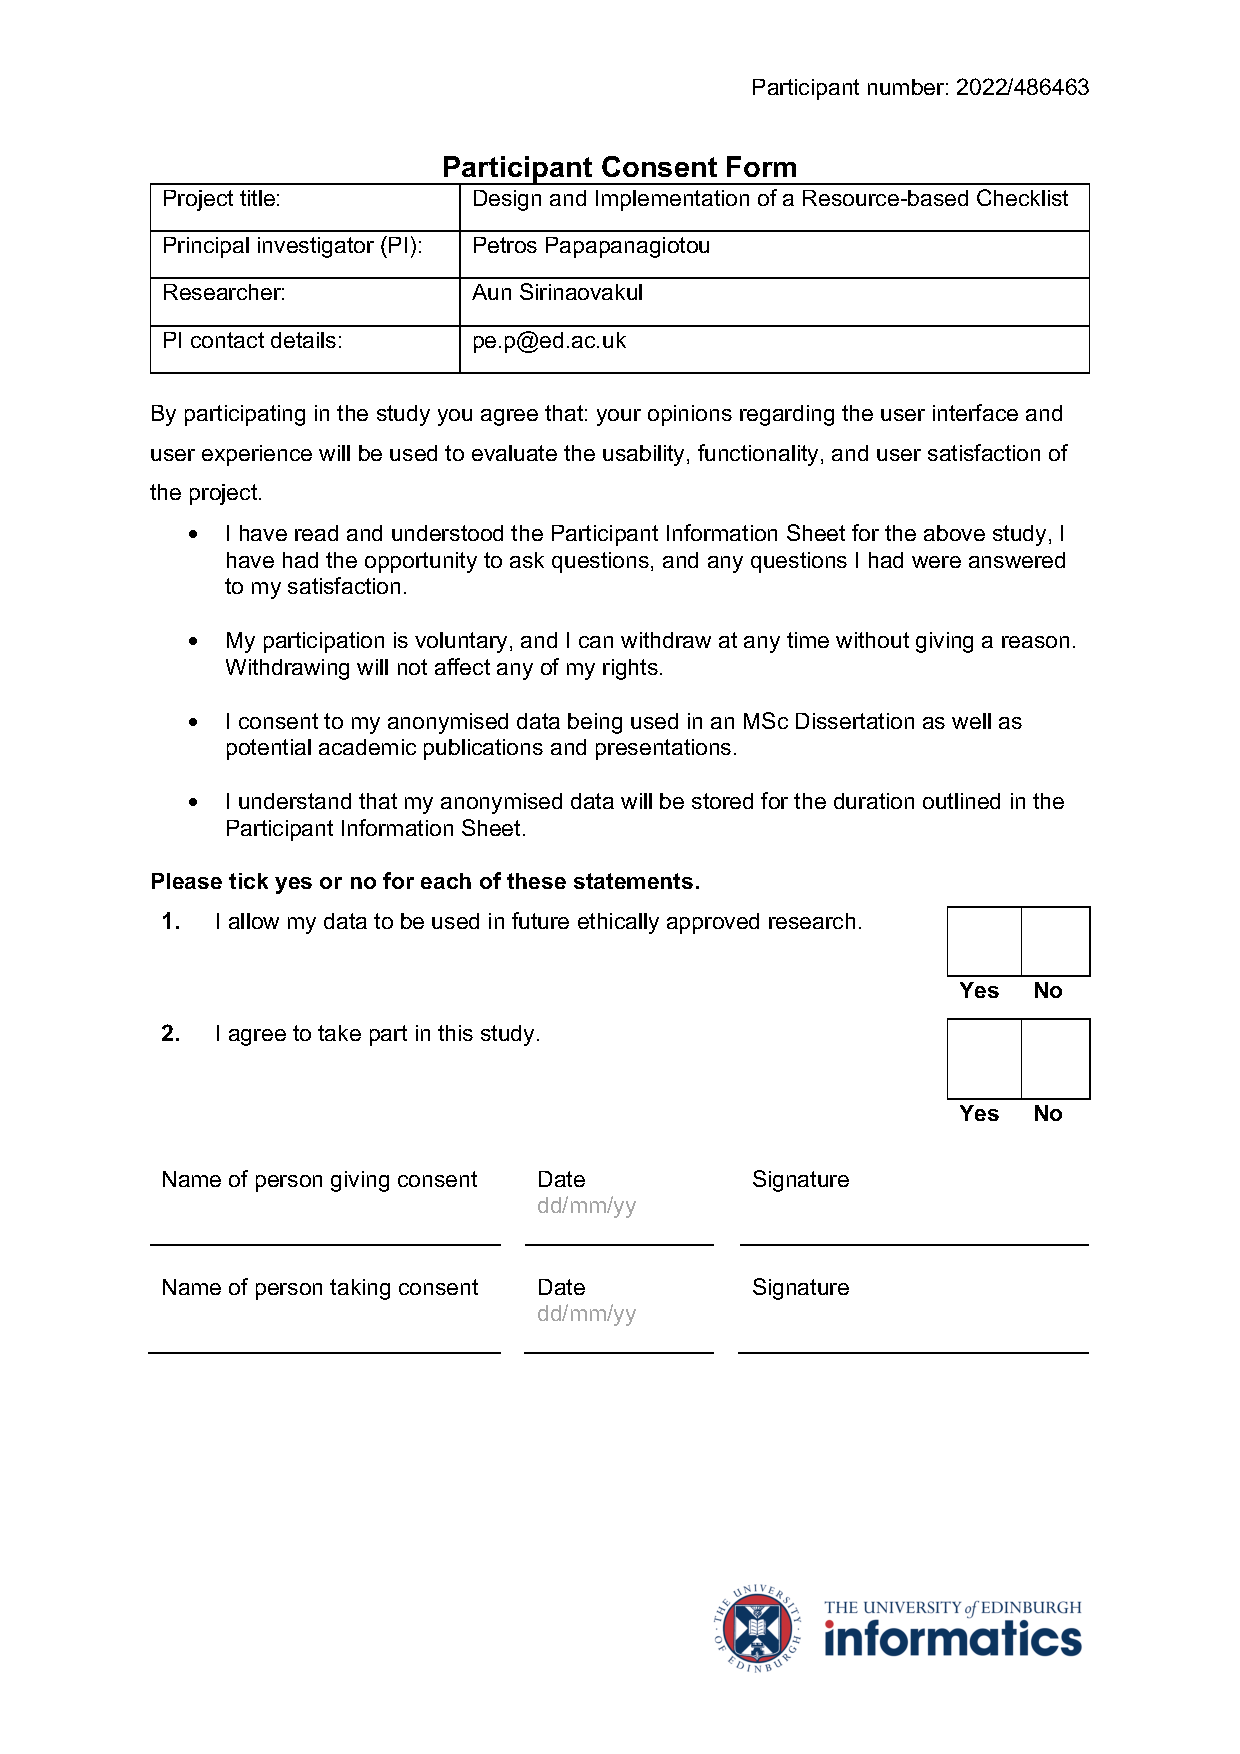
\includepdf[pages=-]{./pdf/Consent Form.pdf}

\chapter{User Evaluation Survey}
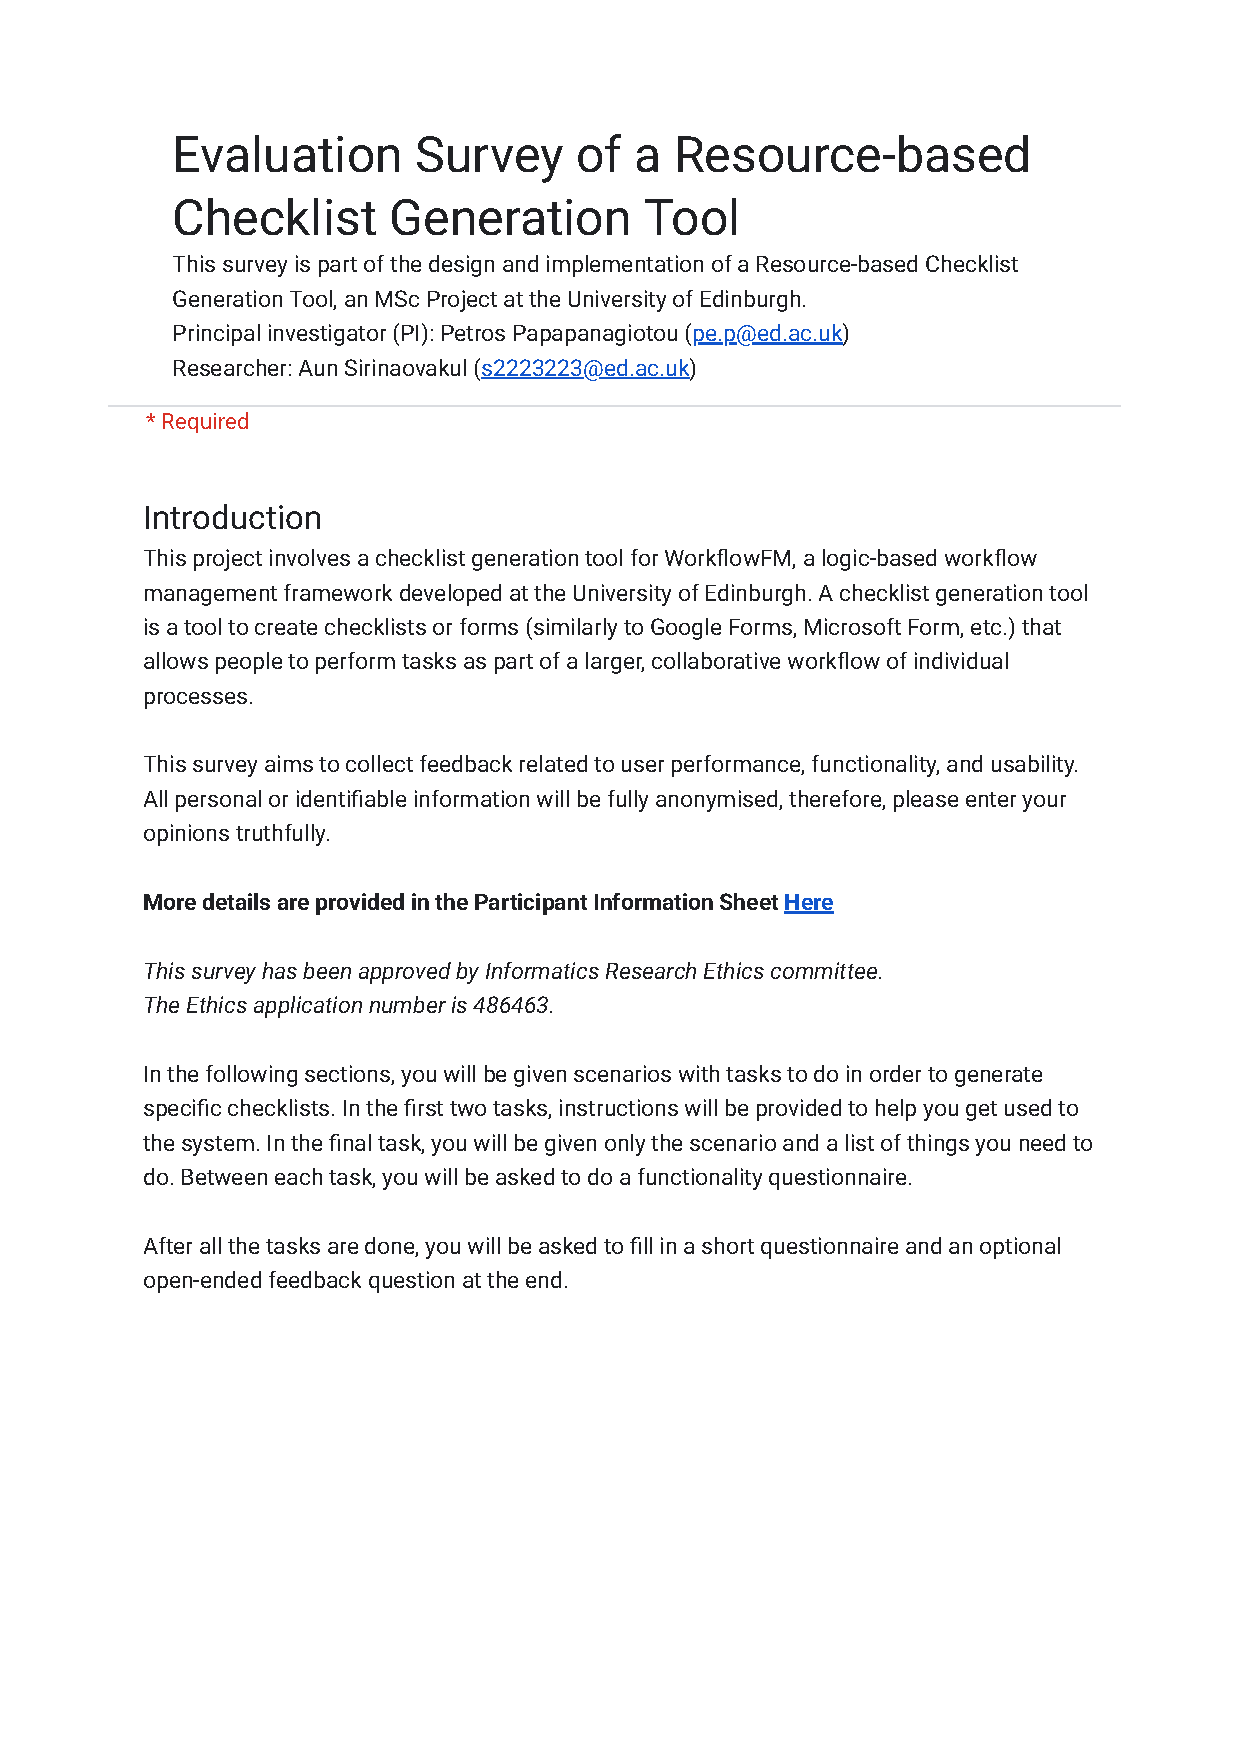
\includepdf[pages=-]{./pdf/Evaluation Survey of a Resource-based Checklist Generation Tool - Google Forms.pdf}
